\section{Theorie}
\label{sec:Theorie}
\subsection{Berechnung der Elektronenbahn im homogenen Magnetfeld}
Die magnetostatische Felder erzeugen Kräfte nur auf die relativ zum Feld bewegte Ladungen. Diese werden als Lorentzkraft bezeichnet $\overrightarrow{\text{F}_{\text{L}}}$
\begin{equation}
    \overrightarrow{\text{F}_{\text{L}}}=\text{q} \cdot \overrightarrow{\text{v}} \cdot \overrightarrow{\text{B}},\\
   \end{equation}
\noindent dabei ist q eine bewegte Ladung mit Geschwindigkeit $\overrightarrow{\text{v}}$ in homogenem magnetischem Feld $\overrightarrow{\text{B}}$.
Es gilt hierbei die Rechte-Hand-Regel mit kartesischen Koordinaten. Ein Elektron (Ladung $\text{e}_0$, Masse $\text{m}_0$) 
bewegt mit Geschwindigkeit $\overrightarrow{\text{v}_0}$ in $\overrightarrow{\text{z}}$-Richtung in homogenem magnetischem Feld $\overrightarrow{\text{B}}$.
 Das magnetische Feld $\overrightarrow{\text{B}}$ hat die Feldlinien in $\overrightarrow{\text{x}}$-Richtung. Sodass erzeugt die Lorentz-Kraft $\overrightarrow{\text{F}_{\text{L}}}$ in $\overrightarrow{\text{y}}$-Richtung
 \begin{align*}
    \text{F}_{\text{Ly}}= \text{e}_0 \text{v}_0 \text{B}.\\
 \end{align*}
 \noindent Unter die Wirkung von $\overrightarrow{\text{F}_{\text{L}}}$ bewegt das Elektron auf einer gekrümmten Bahn in xy-Ebene. 
 Laut (1) ist $\overrightarrow{\text{F}_{\text{L}}}$ senkrecht zum Wegelement d$\overrightarrow{\text{s}}$:
 \begin{align*}
    \overrightarrow{\text{F}_{\text{L}}} \cdot  \text{d}\overrightarrow{\text{s}} = 0,\\
 \end{align*}
 \noindent deswegen ist die pontentielle Energie des Elektrons kontant und daher  ist die kinetische Energie 
 \begin{align*}
    \text{E}_\text{kin} = \frac{1}{2} \text{m}_0 {\text{v}}^2\\
 \end{align*}
 \noindent auch konstant. Der Betrag |$\overrightarrow{\text{v}}$| ist deshalb konstant für alle Bahnpunkte 
 \begin{equation}
    |\overrightarrow{\text{v}}| = \text{v}_0.\\
   \end{equation} 
\noindent Aus dem Gleichgewicht von Lorentzkraft und Zentrifugalkraft
\begin{align*}
    \text{e}_0  \text{v}_0 \text{B} = \frac{\text{m}_0 {|\overrightarrow{\text{v}}|}^2}{\text{r}}\\  
\end{align*}
\noindent wird der Krümmungsradius bestimmt
\begin{equation}
    \text{r} = \frac{\text{m}_0 \text{v}_0 }{\text{e}_0 \text{B }}.\\
\end{equation} 
\noindent Das Elektron bewegt auf einer Kreisbahn, weil der Krümmungsradius laut (3) konstant ist.


\subsection{Experimentelle Bestimmung der spezifischen Elektronenladung}
 Die spezifische Ladung $\text{e}_0/{\text{m}_0}$ der Elektronen kann durch Gleichung (3) bestimmt werden.  Mit einer Katodenstrahlröhre wird einen Elektronenstrahl erzeugt. 
Die kinetische Energie der Elektronen ist gegeben durch:
\begin{align*} 
    \text{E}_{\text{kin}}= \frac{1}{2} \text{m}_0 {\text{v}_0}^2 =  \text{e}_0  \text{U}_\text{B} \\
\end{align*}
\noindent mit $\text{v}_0$ konstante Geschwindigkeit der Elektronen in Achsenrichtung der Röhre und $\text{U}_\text{B}$ das Beschleunigungspotential.
Dann wird $\text{v}_0$ zu
\begin{equation}
    \text{v}_0 = \sqrt{\frac{2 \text{U}_\text{B} \text{e}_0} {\text{m}_0} }.\\  
\end{equation}
\noindent
\begin{figure}[H]
    \begin{center}
    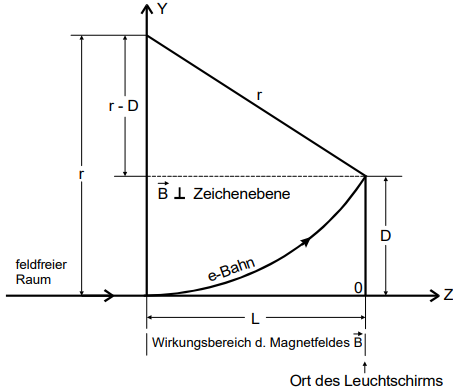
\includegraphics[width = 11cm, height= 10cm]{grafik.png}
    \caption{Skizze zur Ableitung einer Beziehung zwischen L,D und r.\protect\cite{AL}}
    \end{center}
    \label{fig:grafik}
    \end{figure}
    \noindent
Wenn es kein Feld gegeben ist, bewegen sich die Elektronen geradlinig und treffen den Bilschirm auf Mittelpunkt 0 auf und erzeugen dort einen Leuchtfleck.
Wenn der Elektronenstrahl in einem homogenen Magnetfeld B  ausgesetzt (siehe Abbildung \ref{fig:grafik}), wobei auch hier die Bewegungsrichtung der Elektronen und die Feldrichtung senkrecht zueinander sind,  verschiebt sich die Krümmung der Elektronenbahn um das Stück D.
Das Stück D lässt sich einfacher als r messen. 
Der Zusammenhang zwischen D, r und L ist duch den Satz des Pythagoras 
\begin{align*} 
    {\text{L}}^2  + {(\text{r}-\text{D})^2}= {\text{r}}^2 \\
\end{align*}
\noindent gegeben, woraus folgt 
\begin{align*} 
    \text{r} =  \frac{{\text{L}}^2 +{\text{D}}^2 }{2\text{D} }.\\
\end{align*}
\noindent r kann aus (3) eliminiert werden:
\begin{align*} 
    \frac{{\text{L}}^2 +{\text{D}}^2 }{2\text{D} }= \frac{\text{m}_0 \text{v}_0 }{\text{e}_0 \text{B }}.\\
\end{align*}
Durch dem Einsetzen $\text{v}_0$ aus (4) in oberer Gleichung ist die spezifische Ladung $\frac{\text{e}_0}{\text{m}_0}$ der Elektronen bestimmt
\begin{equation}
    \frac{\text{D} }{{\text{L}}^2 +{\text{D}}^2 }  = \frac{1}{\sqrt{8\text{U}_{\text{B}}} } \sqrt{\frac{\text{e}_0}{\text{m}_0}} \text{B}
\end{equation}




